\documentclass[11pt]{article}

\usepackage{amsmath}
\usepackage{amssymb}

\usepackage{graphicx}
\usepackage{tikz}

\usepackage{ytableau}

\title{Partitions, \\ Math 4707, Spring 2021}
\date{}

\begin{document}


\maketitle

\thispagestyle{empty}

\vspace{-0.85cm}

An \emph{(integer) partition} $\lambda = (\lambda_1 \geq \lambda_2 \geq \lambda_3 \ldots)$ is a sequence of weakly decreasing nonnegative integers which is eventually zero. The \emph{size} of $\lambda$ is $|\lambda| := \lambda_1+\lambda_2+...$. The \emph{largest part} of $\lambda$ is $\lambda_1$, and the \emph{length} $\ell(\lambda)$ of $\lambda$ is the number of (nonzero) parts of $\lambda$, i.e., $\ell(\lambda) := \mathrm{max}\{i\colon \lambda_i \neq 0\}$.

The \emph{conjugate} $\lambda'$ of $\lambda$ is the partition whose Young diagram is obtained from that of $\lambda$ by reflecting across the main diagonal:

\vspace{-0.75cm}
\[ \parbox{1.5in}{\begin{center}$\lambda=(3,2,2)$ \\  \ydiagram{3,2,2} \end{center}} \leftrightarrow \parbox{1.5in}{\begin{center} $\lambda'=(3,3,1)$ \\  \ydiagram{3,3,1} \end{center}} \]


\vspace{-0.75cm}

\begin{enumerate}

\item Show that the generating function for partitions with largest part at most $k$ is $\sum_{\lambda\colon \lambda_1 \leq k} q^{|\lambda|} = \prod_{i=1}^{k} \frac{1}{1-q^i}$.
\item Show that the generating function for partitions with length at most $k$ is $\sum_{\lambda\colon \ell(\lambda) \leq k} q^{|\lambda|} = \prod_{i=1}^{k} \frac{1}{1-q^i}$ (hint: use the conjugate).
\item Show that the number of partitions $\lambda$ with largest part at most $a$ and length at most $b$ is $\binom{a+b}{b}$. Hint: think about the following picture (which explains the case $a=4$, $b=3$): 
\vspace{-0.35cm}
\[ \parbox{1in}{$\lambda=(3,2)$\\ \ydiagram{3,2}} \leftrightarrow \qquad \parbox{1in}{ 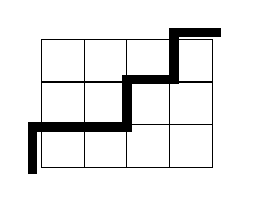
\begin{tikzpicture} \node at (0,0){\ydiagram{4,4,4}};
\def \x {0.6};
\draw[line width=1.2mm, black] (-2*\x,-1.5*\x) -- (-2*\x,-0.5*\x) -- (0*\x,-0.5*\x) -- (0*\x,0.5*\x) -- (1*\x,0.5*\x) -- (1*\x,1.5*\x) -- (2*\x,1.5*\x);
 \end{tikzpicture} } \]
 \item \vspace{-0.35cm} Let $\lambda=(\lambda_1,\lambda_2,\ldots)$ be a partition and $\lambda'=(\lambda'_1,\lambda'_2,\ldots)$ its conjugate. Show that $\sum_{i\geq 1} (i-1) \cdot \lambda_i = \sum_{i\geq 1} \binom{\lambda'_i}{2}$. Hint: think about this picture:
 \vspace{-0.65cm}
\[ \parbox{1.5in}{\begin{center}$\lambda=(3,2,2)$ \\  \begin{ytableau} 0 & 0 & 0 \\ 1 & 1 \\ 2 & 2 \end{ytableau} \end{center}} \leftrightarrow \parbox{1.5in}{\begin{center} $\lambda'=(3,3,1)$ \\  \begin{ytableau} 0 & 1 & 2 \\ 0 & 1 & 2 \\ 0  \end{ytableau}  \end{center}}  \vspace{-0.15cm} \]

\item \vspace{-0.45cm} Describe the partition $\lambda$ of size $|\lambda|=n$ which maximizes $\mathrm{min}(\lambda_1,\ell(\lambda))$.

\end{enumerate}

\end{document}
